\documentclass[12pt]{article}
\title{M374M Homework 3 \\
  \normalsize{\S~1.3 \#1a, 1n, 8a$^1$, 9, 13}}
\author{Hershal Bhave (hb6279)}
\date{Due 2016--02--15}

\usepackage{macros}

\begin{document}
\maketitle

\section{\S~1.3}
\subsection{1a, 1n}
\subsubsection*{Problem}
Find the general solution of the following differential equations:
\begin{enumerate}
\item $u'+2u=e^{-t}$
\item $u''+\omega^2u=\cos\omega t$
\end{enumerate}

\subsubsection*{Solution}
\begin{enumerate}
\item This first-order ODE may be rewritten is in standard form
  \begin{equation}
    \label{eq:1a-standard-form}
    \od{u}{t} + p(t)u = q(t),
  \end{equation}
  where $p(t)=2$ and $q(t)=e^{-t}$. This ODE may be solved by obtaining an
  integrating factor $r$.
  \begin{equation*}
    \label{eq:1a-integrating-factor}
    \begin{aligned}
      r(t) &= e^{\int p(t) \dd{t}} \\
      &=e^{2t} \\
    \end{aligned}
  \end{equation*}
  Multiplying both sides of \cref{eq:1a-standard-form} by $r$ yields
  $$\od{u}{t} e^{2t} + 2u e^{2t} = e^{-t} e^{2t}$$
  or \todo[why does $p(t)r(t)u$ disappear?]
  $$\od{}{t}(u e^{2t}) = e^{t}.$$
  Integrating both sides yields
  \begin{equation} \boxed{
    \begin{aligned}
      u e^{2t} &= \int e^{t}\dd{t} = e^{t} + C \\
      \implies u &= e^{-t} + C e^{-2t} \\
    \end{aligned}
    }
  \end{equation}

\item The general form of a second-order ODE is
  $$P(t)\od[2]{u}{t} + Q(t)\od{u}{t} + R(t)u = G(t)$$

  The general solution to a second-order ODE is $$u = u_c + u_p$$ where $u_c$ is
  the solution to the homogenous case ($G=0$) and $u_p$ is a particular
  solution.

  In the homogenous case
  $$u''+\omega^2u=0,$$
  which may be transformed into the characteristic equation
  $$r^2+\omega^2=0.$$

  Solving this results in $r=\pm i\omega$ so that the complementary equation
  takes the form.
  \begin{equation}
    \label{eq:1n-hom-sol}
    \implies u_c = c_1e^{i\omega t}c_2e^{-i\omega t}
  \end{equation}

  In our case, the particular solution takes the form\footnote{The $t$ appears
    at the end of the general solution to ensure uniqueness since a similar form
    exists in $G(t)$.}
  \begin{equation*}
    \begin{aligned}
      u_p(t) &= (A\cos \omega t + B\cos \omega t)t \\
      &= (At\cos \omega t + Bt\sin \omega t) \\
    \end{aligned}
  \end{equation*}

  Substituting this into the the original equation yields
  \begin{equation}
    \label{eq:1n-undetermined-coefs}
    \begin{aligned}
      \cos \omega t &=
      \od[2]{u}{t}(At\cos \omega t + Bt\sin \omega t)
      + ((At\cos \omega t + Bt\sin \omega t)t)\omega^2 \\
      &= (2B\omega - \cancel{A\omega^2t})\cos\omega t
      + (-2A\omega - \cancel{B\omega^2t})\sin\omega t
      + \cancel{A\omega^2t\cos\omega t} + \cancel{B\omega^2t\sin\omega t} \\
      &= 2B\omega\cos\omega t - 2A\omega\sin\omega t.
    \end{aligned}
  \end{equation}
  From \cref{eq:1n-undetermined-coefs}, we may conclude that $A=0$ and
  $B=1/2\omega$.
  \begin{equation}
    \label{eq:1n-nonhom-sol}
    \implies u_p = \frac{t}{2\omega}\sin\omega t
  \end{equation}
  Finally, we may assemble the general solution from
  \cref{eq:1n-hom-sol,eq:1n-nonhom-sol}.
  \begin{equation*}
    \boxed{
      u = c_1e^{i\omega t}c_2e^{-i\omega t} + \frac{t}{2\omega}\sin\omega t
    }
  \end{equation*}
\end{enumerate}

\subsection{8a$^1$}
\subsubsection*{Problem}
The model in \cref{eq:8a-problem} contains a parameter $h$. Find equilibria in
terms of $h$ and determine their stability. Construct a bifurcation diagram
showing how equilibria depend upon $h$, and label the branches of the curves as
stable or unstable.

\begin{equation}
  \label{eq:8a-problem}
  u'=hu-u^2
\end{equation}

\subsubsection*{Remarks}
Assume the parameter $h$ may take any value: negative, zero, or positive.

\subsubsection*{Solution}
By inspection, the equilibria for this problem are $u_*=0,\,h$. We will
enumerate through the solutions and use the derivative method to establish the
stability of the equilibrium solutions.
\begin{enumerate}
\item $u_*=0$.
  $$\implies u''=h.$$ From this, we may conclude that $u_*$ is stable if $h<0$
  and is unstable if $h\ge0$.
\item $u_*=h$.
  $$\implies u''=-h$$ From this, we may conclude that $u_*$ is unstable if $h\le0$
  and is stable if $h>0$.
\end{enumerate}
Reference the bifurcation diagram in \cref{fig:8-bifurcation-diagram}.

\begin{figure}
  \centering
  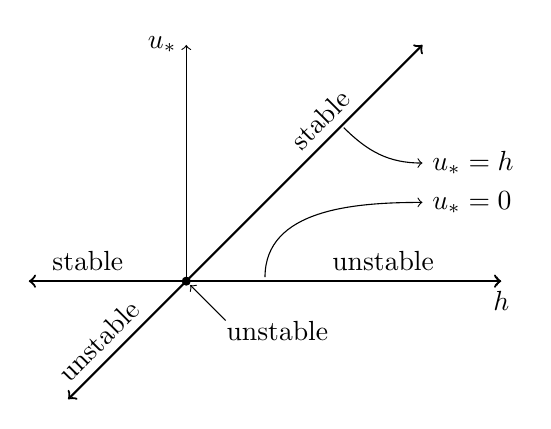
\begin{tikzpicture}
    %% axes
    \draw[<->] (0,3) node [left] {$u_*$} -- (0,0) -- (4,0) node [below] {$h$};
    %% lines
    \draw[thick,<->] (-2,0) -- (4,0)
    node[very near start,above]{stable}
    node[near end,above]{unstable};
    \draw[thick,<->] (-1.5,-1.5) -- (3,3)
    node[very near start,above,sloped]{unstable}
    node[near end,above,sloped]{stable};
    \draw[fill] (0,0) circle [radius=0.05];
    \draw[<-] (0.05,-0.05) -- (0.5,-0.5) node[near end,below right]{unstable};

    \draw[->] (1,0.05) to [out=90,in=180] (3,1) node[right]{$u_*=0$};
    \draw[->] (2,1.95) to [out=-45,in=180] (3,1.5) node[right]{$u_*=h$};
  \end{tikzpicture}
  \caption{Bifurcation diagram for \#8}
  \label{fig:8-bifurcation-diagram}
\end{figure}

\subsection{9}
\subsubsection*{Problem}
Consider the model
\begin{equation}
  \label{eq:9-problem}
  u'=(\lambda - b) u-au^3,
\end{equation}
where $a$ and $b$ are fixed positive constants and $\lambda$ is a parameter that
varies.

\begin{enumerate}
\item If $\lambda < b$  show that there is a single equilibrium and that it is
  asymptotically stable.
\item If $\lambda > b$ find all equilibria and determine their stability
\item Sketch the bifurcation diagram showing how equilibria vary with $\lambda$.
  Label each branch of the curves shown in the bifurcation diagram as stable or
  unstable.
\end{enumerate}

\subsubsection*{Solution}
\todo[]

\subsection{13}
\subsubsection*{Problem}
A one-dimensional system is governed by the dynamical equation
\begin{equation}
  \label{eq:13-problem}
  u'-4u(a-u)-he^{-u}
\end{equation}
where $a$ and $h$ are positive constants. Draw a bifurcation diagram with
respect to the parameter $a$ while holding $h$ constant. Indicate the stable and
unstable branches.

\subsubsection*{Solution}
\todo[]

\newpage
\section{Programming Minilab}
A simple model for the population of plants in a plant-herbivore ecosystem is
\begin{equation}
  \label{eq:minilab-problem}
  \od{p}{t} = rp\left( 1-\frac{p}{k} \right) - \frac{apq}{1+bp}, \quad p(0)=p_0
\end{equation}
Here $p(t)$ is the number of plants, $q$ is the constant number of herbivores,
$r$ and $k$ are constants that describe the growth rate of the plants, and $a$
and $b$ are constants that describe the consumption rate of the plants by the
herbivores. Here we perform a qualitative analysis to understand the behavior of
solutions of the model in \cref{eq:minilab-problem}. To quantify the population
sizes we introduce the dimensions $[p] = \text{Plant}$, $[q] =
\text{Herbivore}$, and $[t] = \text{Time}$. All constants are assumed positive.

\subsubsection*{Problem}
\begin{enumerate}
\item Find the dimensions of $r$, $k$, $a$, and $b$. Using the scales $t_c =
  1/r$ and $p_c = k$, show that the dimensionless version of
  \cref{eq:minilab-problem} takes the form
  \begin{equation}
    \label{eq:minilab-problem-a}
    \od{u}{\tau}=u(1-u)-\frac{hu}{1+cu},\quad u(0)=u_0
  \end{equation}
  where $u=p/p_c$, $\tau=t/t_c$, and $h,c$ are constants which you should
  identify.
\item Assuming $c>1$ is fixed, find (or characterize) all equilibrium solutions
  of \cref{eq:minilab-problem-a} and determine their stability in terms of the
  parameter $h>0$. Illustrate the results on a bifurcation diagram.
\label{item:minilab-part-b}
\item Use \verb|program3.m| and \verb|plant.m| to numerically simulate the model
  in \cref{eq:minilab-problem-a}. Produce portraits of solutions for various
  $u_0$ when $c=4$ and a few different values of $h$. Do the simulations agree
  with the analysis in \cref{item:minilab-part-b}? According to the stability
  results in the bifurcation diagram, do solutions grow, decay, or remain
  constant?
\item For what range of the parameter $h$ would the plant population survive if
  $\tau\rightarrow\infty$, $c=4$, and $u(0)=1/4$? For what range of $h$, if any,
  would the plant population die out as $\tau\rightarrow\infty$?
\end{enumerate}

\subsubsection*{Solution}
\todo[]

\end{document}
